\documentclass[10pt,a4paper]{article}
\usepackage[utf8]{inputenc}
\usepackage{amsmath}
\usepackage{amsfonts}
\usepackage{amssymb}
\usepackage{graphicx}
\usepackage{caption}
\usepackage{sidecap}
\usepackage{framed}
\usepackage{subcaption}
\usepackage[textwidth=13cm, textheight=22cm]{geometry}
\usepackage{todonotes}

\title{Report Multi-agent Systems Module II}
\author{Tom Jacobs (s0214835), Thomas Uyttendaele (s0215028)}
\begin{document}
\maketitle

%%%%%%%%%%%%%%%%%%%%%%%%%%%%%%%%%%%%%%%%%%%%%
%											%
%					Part I					%
%											%
%%%%%%%%%%%%%%%%%%%%%%%%%%%%%%%%%%%%%%%%%%%%%

\part{}

%%%%%%%%%%%%%%%%%%%%%%%%%%%%%%%%%%%%%%%%%%%%%
%											%
%				Value Iteration				%
%											%
%%%%%%%%%%%%%%%%%%%%%%%%%%%%%%%%%%%%%%%%%%%%%

\section{Value iteration in MDPs}

The different implementations of Value Iteration have been verified using the $Q^{*}$ provided for the \emph{loadunload} problem. They match exactly within the accuracy of the reference matrix.

\subsubsection*{Rewards}

The average sums of discounted rewards and relevant standard deviations (between parenthesis) have been visualised in \ref{table:rewards}. 
They are the result of 100 runs with a horizon of 100 steps.
The results for \emph{MLS} and \emph{$Q_{MDP}$} will be further discussed in the next section.

A brief comparison between the results for the \emph{Initial Start Distribution} and the \emph{Fully Observable} implementations shows that the latter produces slightly smaller reward values. 
The main reason is that a horizon chosen at 100 steps still somewhat limits the maximal achievable reward.

\subsubsection*{Performance statistics}

The algorithm for \emph{Value Iteration} presented in the slides was implemented with a few minor modifications for performance reasons. 
Looping is first done over actions and then nested the different states. To exploit the sparsity of some of the matrices the Matlab \emph{find()} function is used.

To optimize the calculation of the $Q^{*}$ matrices a second implementation was done where the fetching of the non-zero elements from sparse matrices is done up front. 
The average running time and standard deviation of running times in seconds for \emph{Value Iteration} can be found in table \ref{table:vi}.
Here the new algorithm is the modified version with fetching before the actual loops.
\begin{framed}
\textit{note: for all timing results presented in this report the first value is removed before processing, as it is usually an outlier due to initialization and caching delays.}
\end{framed}
\newpage

%%%%%%%%%%%%%%%%%%%%%%%%%%%%%%%%%%%%%%%%%%%%%
%											%
%					Tables					%
%											%
%%%%%%%%%%%%%%%%%%%%%%%%%%%%%%%%%%%%%%%%%%%%%

\begin{table}
\centering
\begin{tabular}{ c || c | c || c | c}
Problem & $\mu_{Old}$ & $\mu_{New}$ & $\sigma_{Old}$ & $\sigma_{New}$ \\
\hline
loadunload & 3.744e-02 & 3.213e-02 & 1.035e-03 & 1.305e-03\\
hallway & 7.463e-01 & 7.167e-01 & 1.0582e-02 & 9.933e-03\\
hallway2 & 1.167e+00 & 1.115e+00 & 1.024e-02 & 9.640e-03 \\
trc & 1.396e+01 & 1.367e+01 & 3.102e-01 & 2.993e-01\\
\end{tabular}
\caption{Value Iteration runtime statistics for both algorithms}
\label{table:vi}
\end{table}

\begin{table}
\centering
\begin{tabular}{ c || c | c | c | c }
\hfill & Initial Start & Fully & MLS & $Q_{MDP}$\\
\hfill & Distribution &  Observable &  & \\
\hline
hallway & 1.536 & 1.521 (0.5654) & 0.8552 (0.3829) & 0.3066 (0.3750) \\
hallway2 & 1.201 & 1.179 (0.4823) & 0.1896 (0.1688) & 0.09883 (0.2166)\\
trc & 10.89 & 10.54 (2.808) & 4.634 (2.524) & 0 (0)
\\
\end{tabular}
\caption{Reward values for the different algorithms}
\label{table:rewards}
\end{table}

%%%%%%%%%%%%%%%%%%%%%%%%%%%%%%%%%%%%%%%%%%%%%
%											%
%					Figures					%
%											%
%%%%%%%%%%%%%%%%%%%%%%%%%%%%%%%%%%%%%%%%%%%%%

\begin{SCfigure}
\vspace{-20pt}
\hspace{-30pt}
\centering
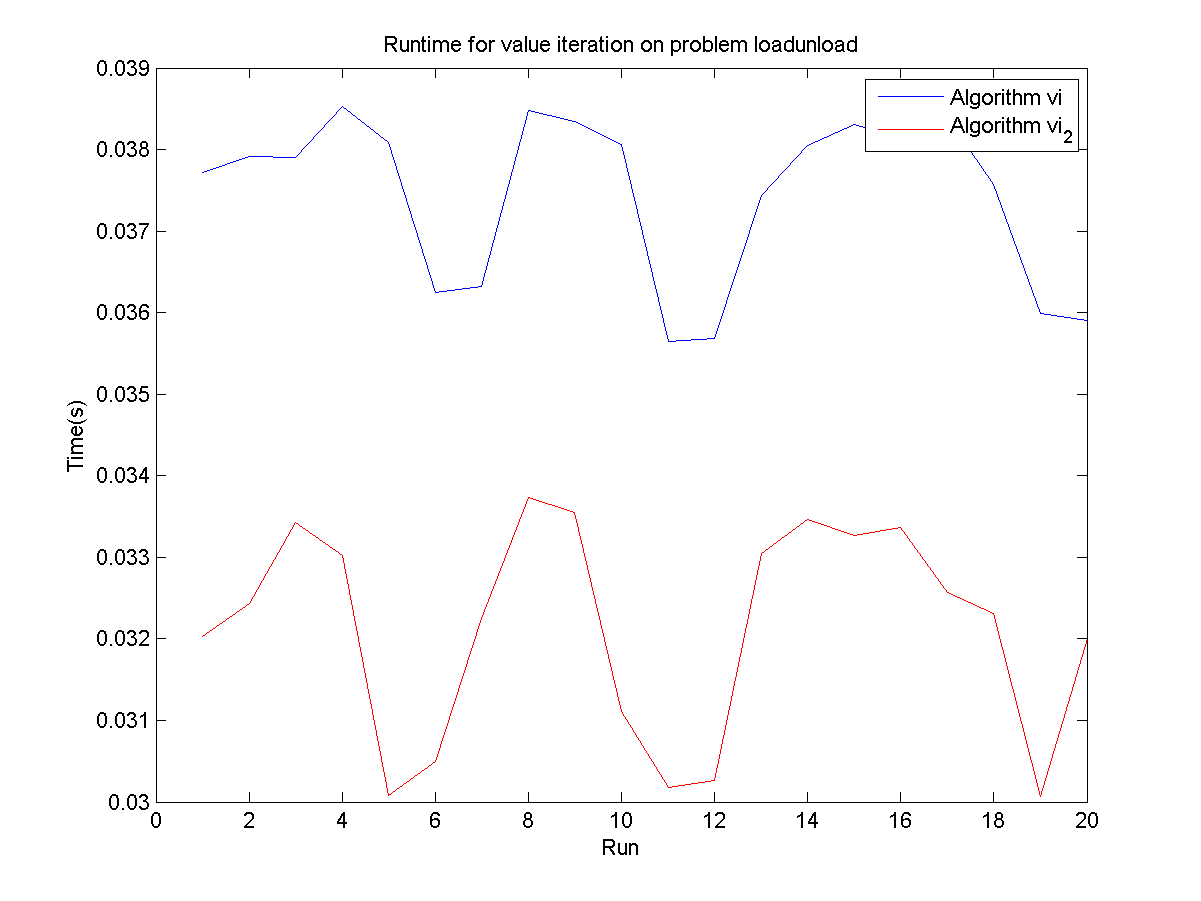
\includegraphics[width=0.7\textwidth]{Timings/loadunload/timings_vi.png}
\hspace{-30pt}
\caption{The loadunload problem}
\label{fig:vi_loadunload}
\vspace{-20pt}
\end{SCfigure}

\begin{SCfigure}
\vspace{-20pt}
\hspace{-30pt}
\centering
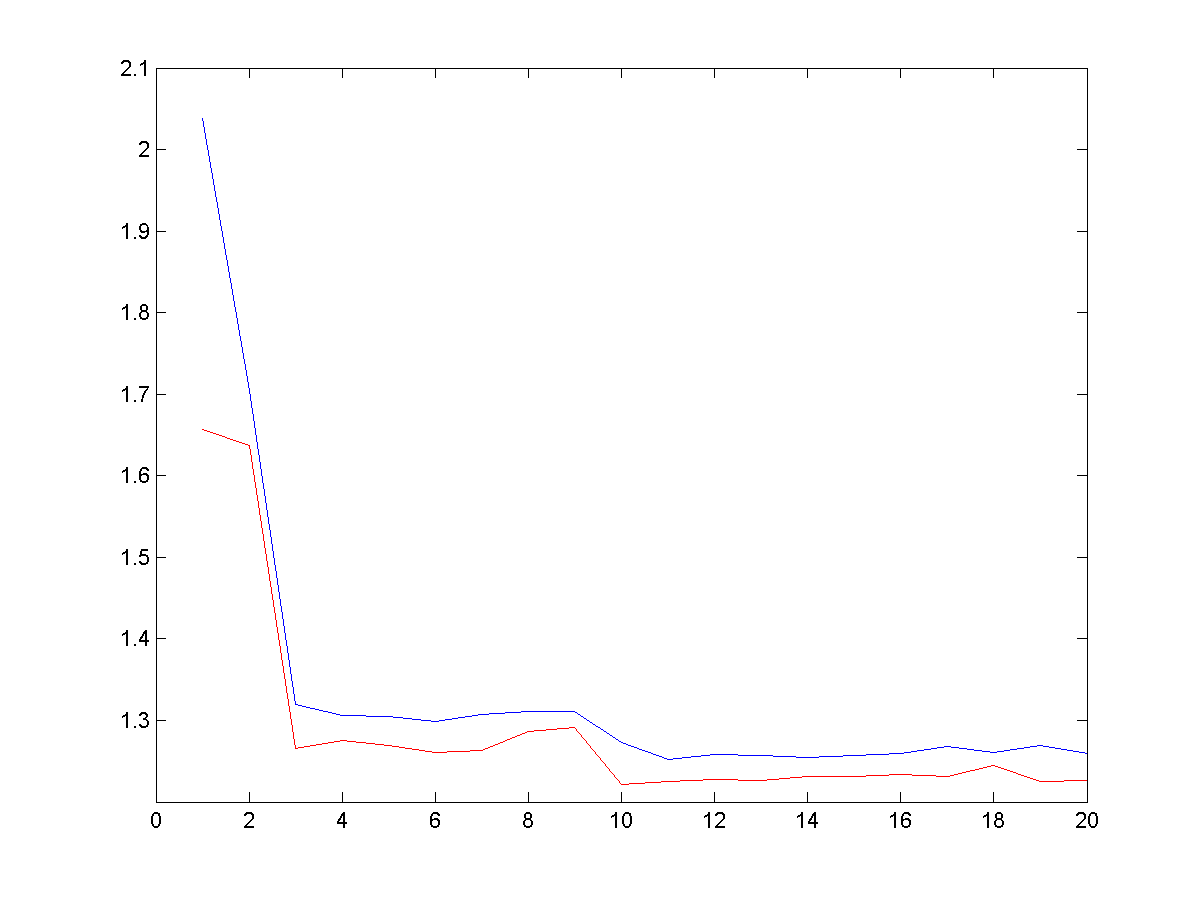
\includegraphics[width=0.7\textwidth]{Timings/hallway/timings_vi.png}
\caption{The hallway problem}
\hspace{-30pt}
\label{fig:vi_hallway}
\vspace{-20pt}
\end{SCfigure}
        
\begin{SCfigure}
\vspace{-20pt}
\hspace{-30pt}
\centering
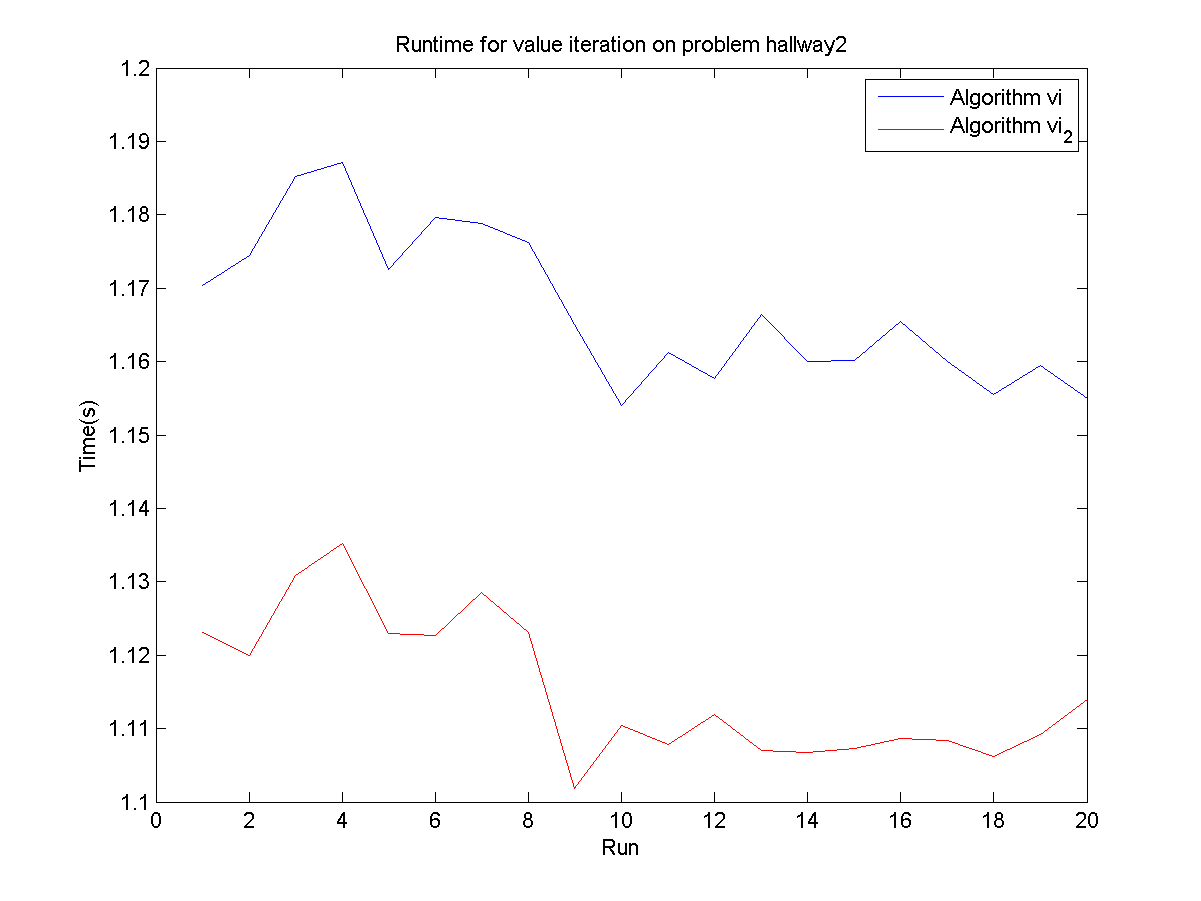
\includegraphics[width=0.7\textwidth]{Timings/hallway2/timings_vi.png}
\caption{The hallway2 problem}
\hspace{-30pt}
\label{fig:vi_hallway2}
\vspace{-20pt}
\end{SCfigure}
        
\begin{SCfigure}
\vspace{-20pt}
\hspace{-30pt}
\centering
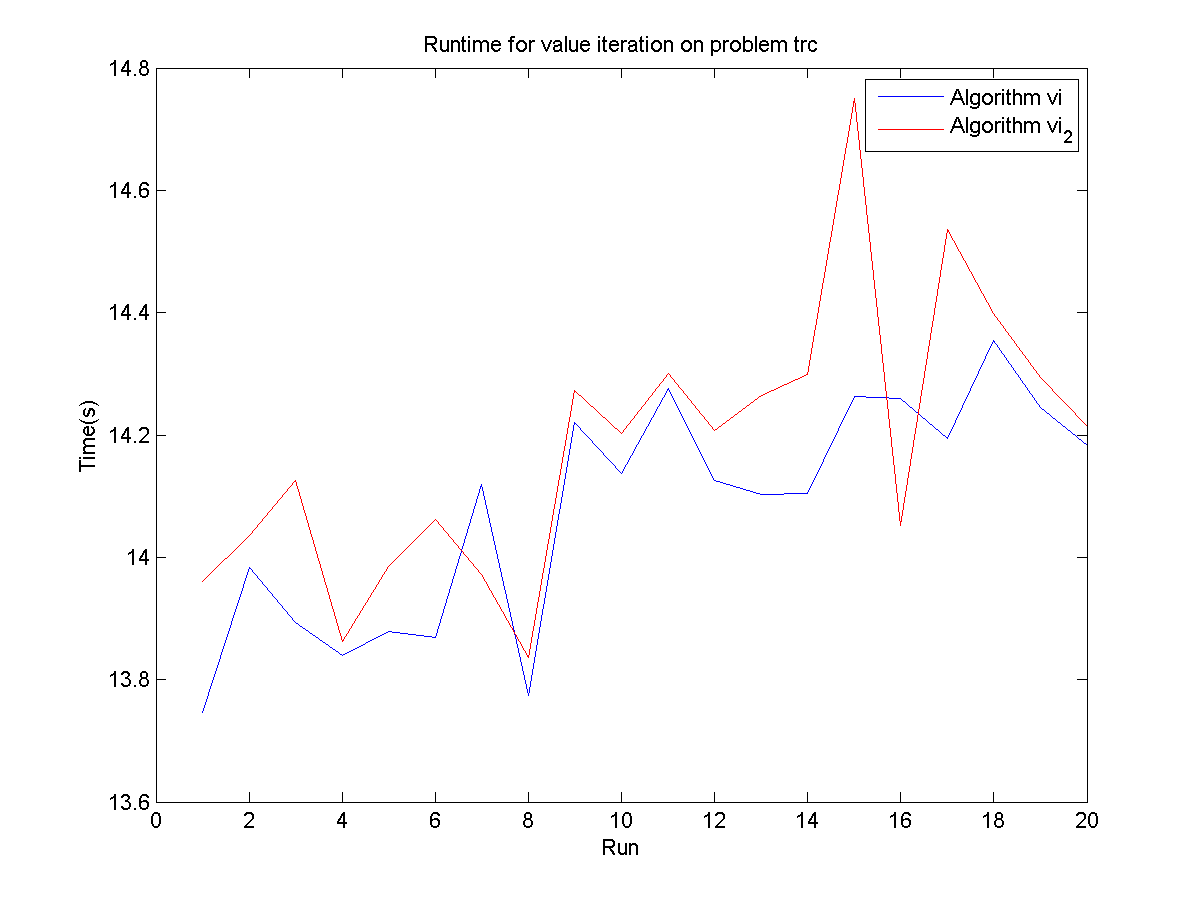
\includegraphics[width=0.7\textwidth]{Timings/trc/timings_vi.png}
\hspace{-30pt}
\caption{The trc problem}
\label{fig:vi_trc}
\vspace{-20pt}
\end{SCfigure}

%%%%%%%%%%%%%%%%%%%%%%%%%%%%%%%%%%%%%%%%%%%%%
%											%
%					Paths					%
%											%
%%%%%%%%%%%%%%%%%%%%%%%%%%%%%%%%%%%%%%%%%%%%%

\subsubsection*{Paths followed}

In figures \ref{fig:path_hallway} and \ref{fig:path_trc} a path followed in the hallway and trc problem is visualized.
This is done by first displaying the respective state and using the height of the bars or darkness of the circles to show the continuation in time. 
If a state is visited multiple times the last visit is drawn.

The figures marked (b) show which states are visited throughout the run itself.

\newgeometry{textwidth=16cm, textheight=25cm}
\begin{figure}
        \centering
        \begin{subfigure}{0.48\textwidth}
                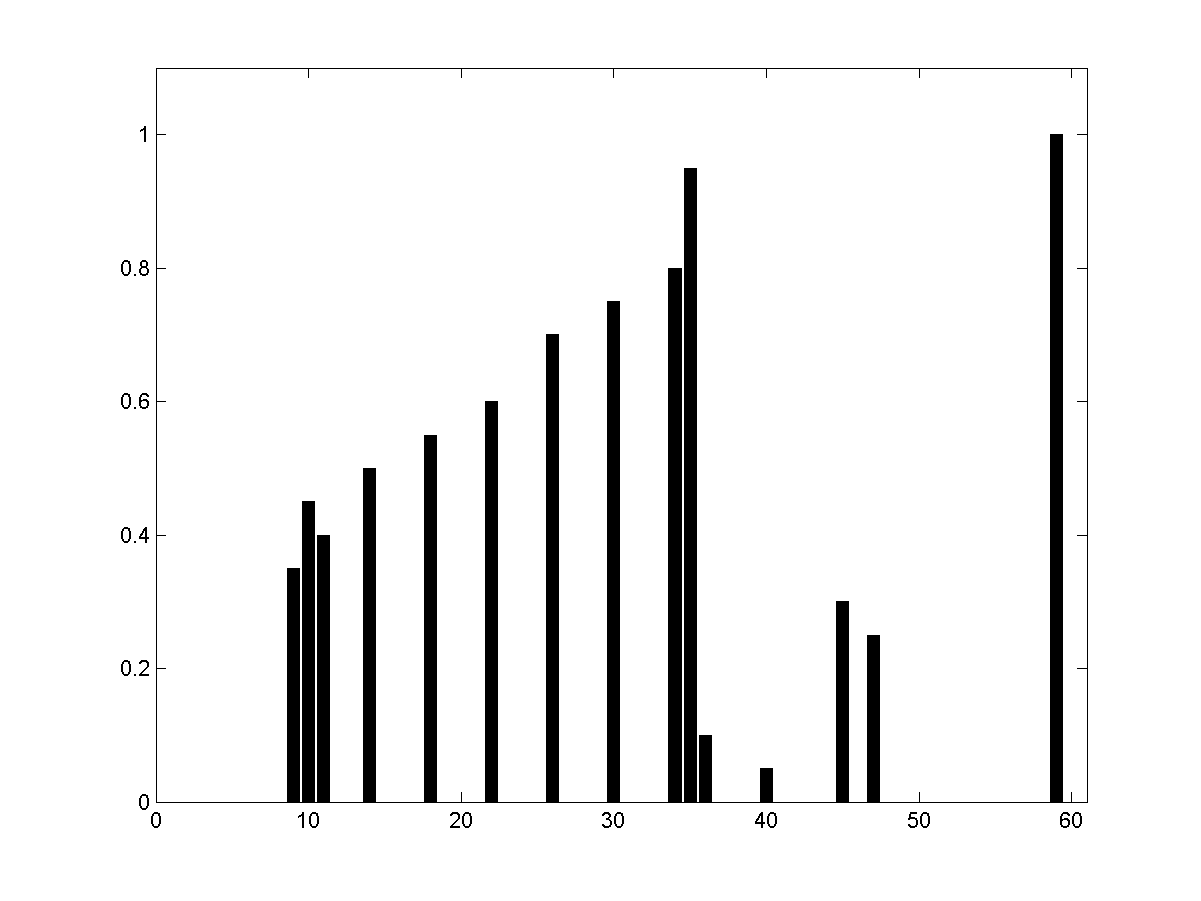
\includegraphics[width=\textwidth]{Paths/hallway/plot-basic-part1-4096896640.png}
                \caption{Last time in state, higher means more recent}
                \label{fig:path_hallway_part1}
                \hspace{10pt}
        \end{subfigure}
        \quad
        \begin{subfigure}{0.48\textwidth}
        		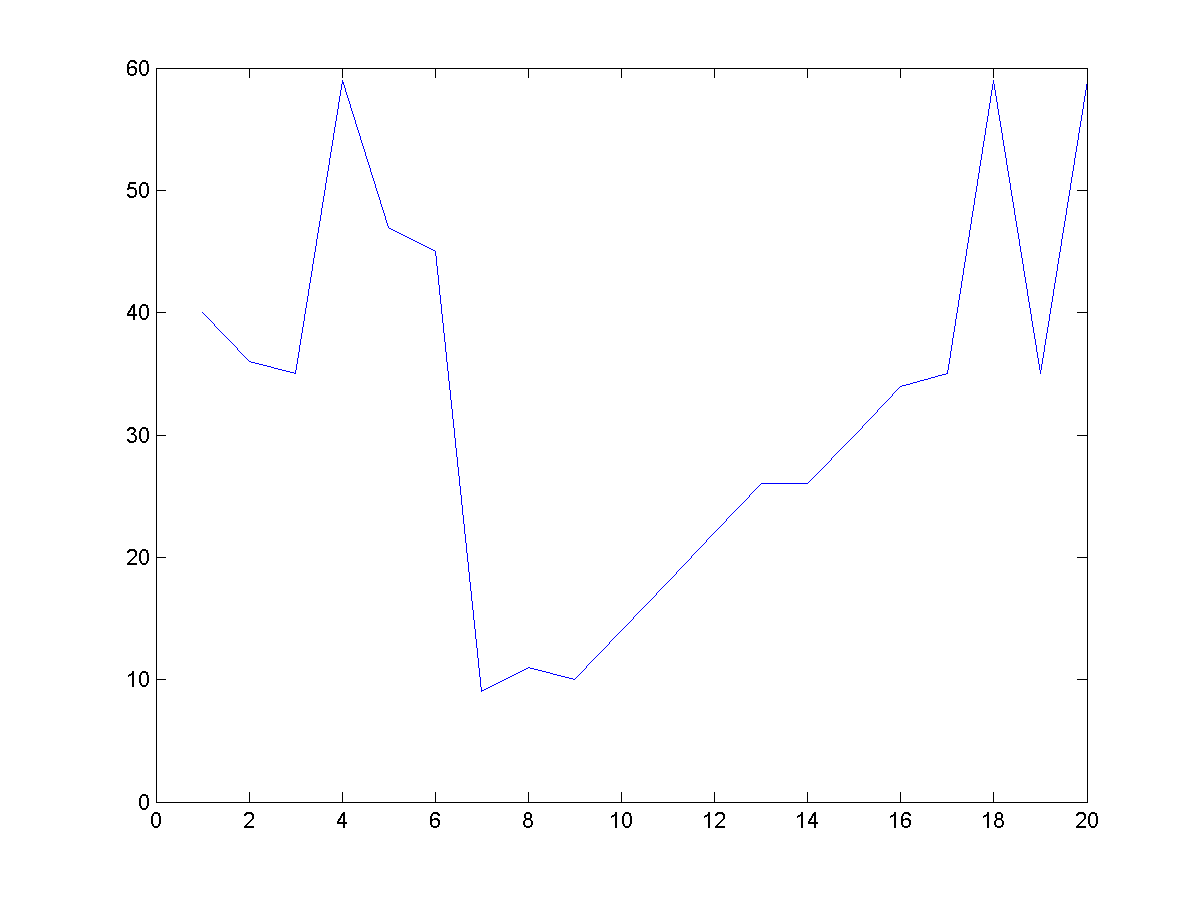
\includegraphics[width=\textwidth]{Paths/hallway/plot-basic-part2-4096896640.png}
                \caption{Run through the states}
                \label{fig:path_hallway_part2}
                \hspace{-10pt}
        \end{subfigure}
        \caption{A path through the hallway problem}
        \label{fig:path_hallway}
\end{figure}

\begin{figure}
        \centering
        \begin{subfigure}{0.48\textwidth}
        		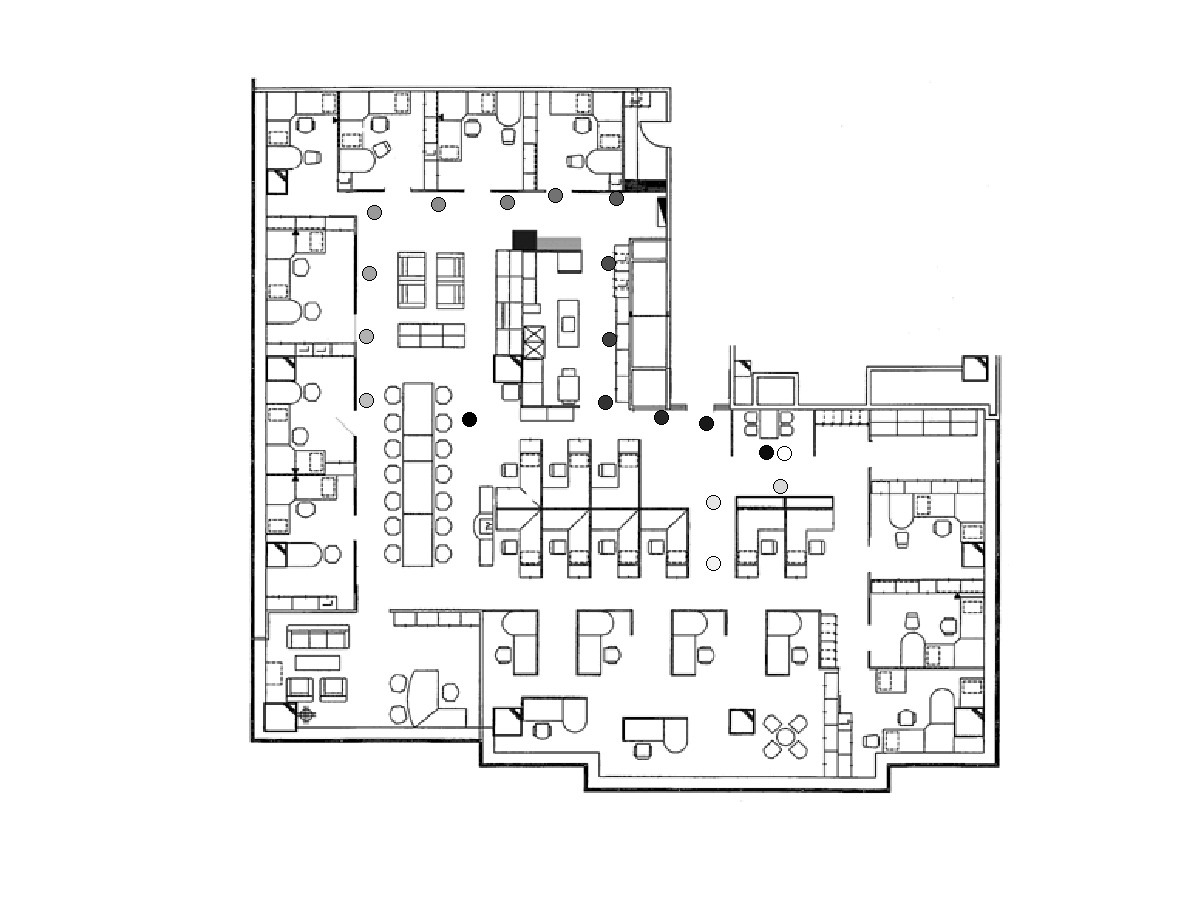
\includegraphics[width=\textwidth]{Paths/trc/plot-basic-part1-6129604379.png}
                \caption{Last time in state, darker means more recent}
                \label{fig:path_trc_part1}
                \hspace{10pt}
        \end{subfigure}
        \quad
        \begin{subfigure}{0.48\textwidth}
        		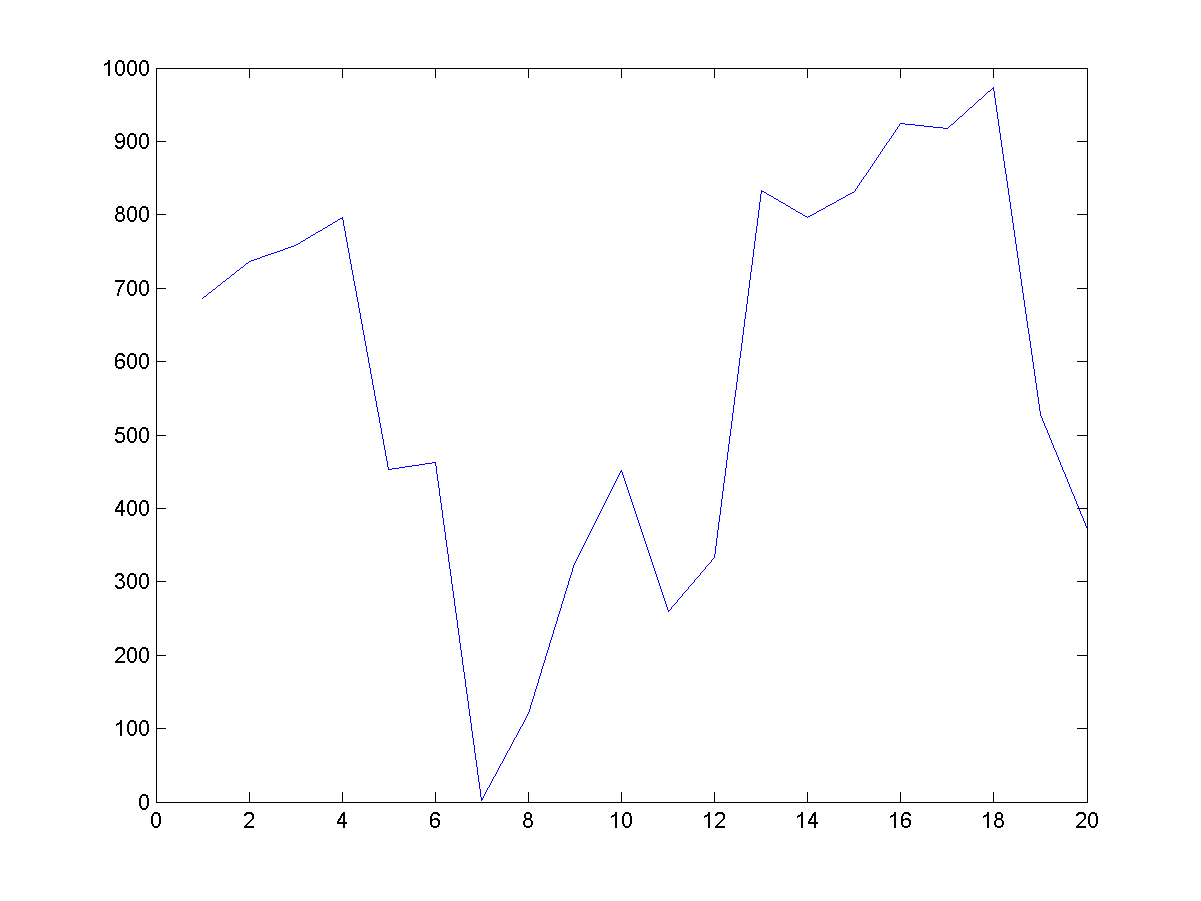
\includegraphics[width=\textwidth]{Paths/trc/plot-basic-part2-6129604379.png}
                \caption{Run through the states}
                \label{fig:path_trc_part2}
                \hspace{-10pt}
        \end{subfigure}
        \caption{A path through the trc problem}
        \label{fig:path_trc}
\end{figure}

\begin{figure}
        \centering
        \begin{subfigure}{0.48\textwidth}
        		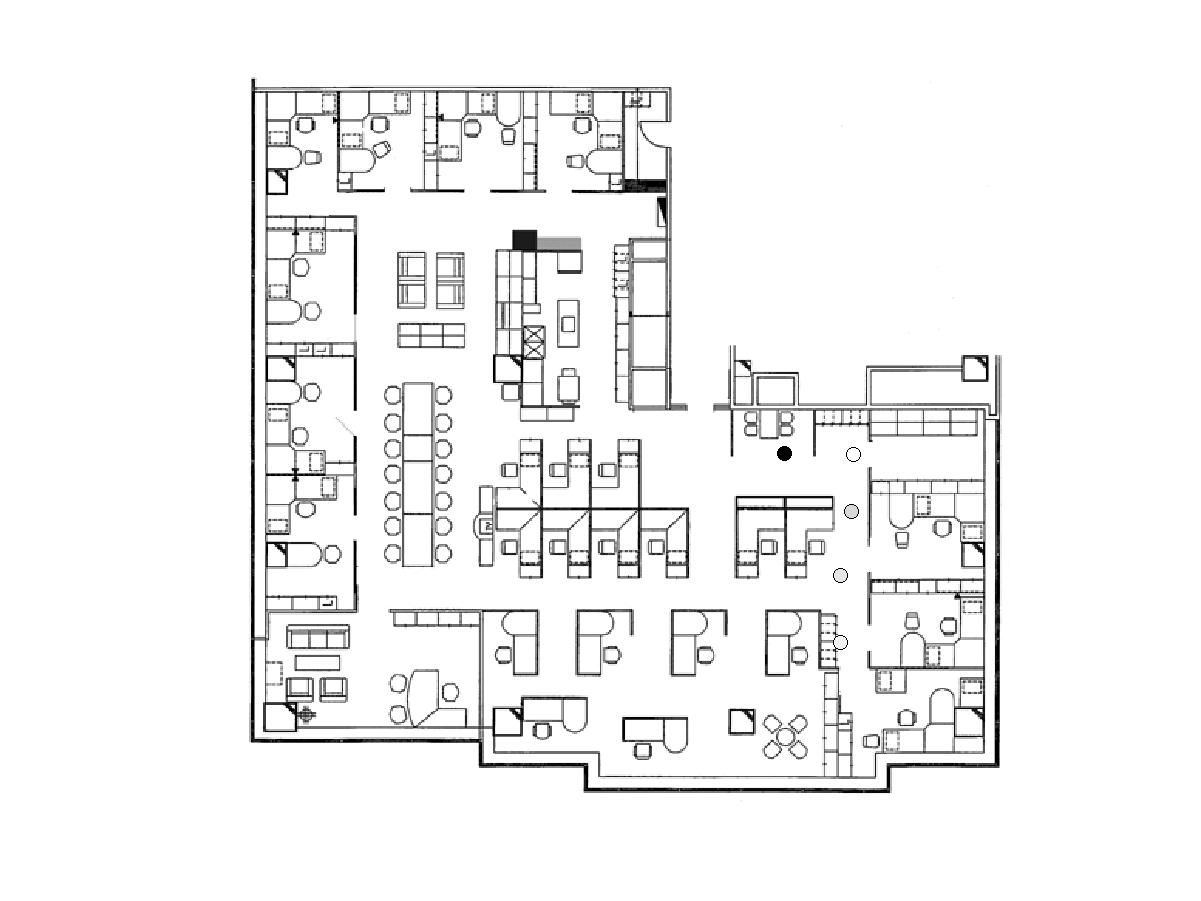
\includegraphics[width=\textwidth]{Paths/trc/plot-QMDP-part1-7002556633.png}
                \caption{Last time in state, darker means more recent}
                \label{fig:path_trc_part1}
                \hspace{10pt}
        \end{subfigure}
        \quad
        \begin{subfigure}{0.48\textwidth}
        		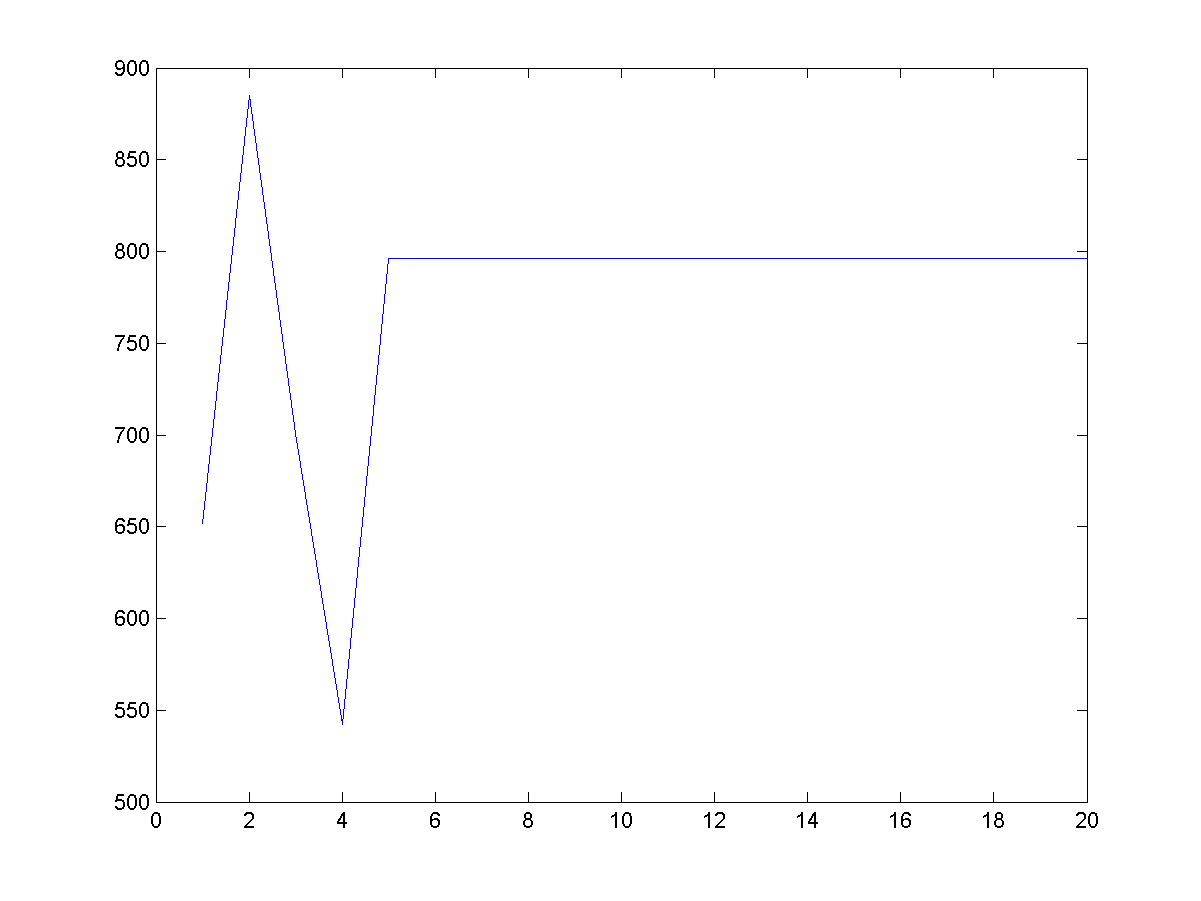
\includegraphics[width=\textwidth]{Paths/trc/plot-QMDP-part2-7002556633.png}
                \caption{Run through the states}
                \label{fig:path_trc_part2}
                \hspace{-10pt}
        \end{subfigure}
        \caption{The trc problem during a $Q_{MDP}$ run}
        \label{fig:trc_qmdp}
\end{figure}

\begin{figure}
        \centering
        \begin{subfigure}{0.48\textwidth}
        		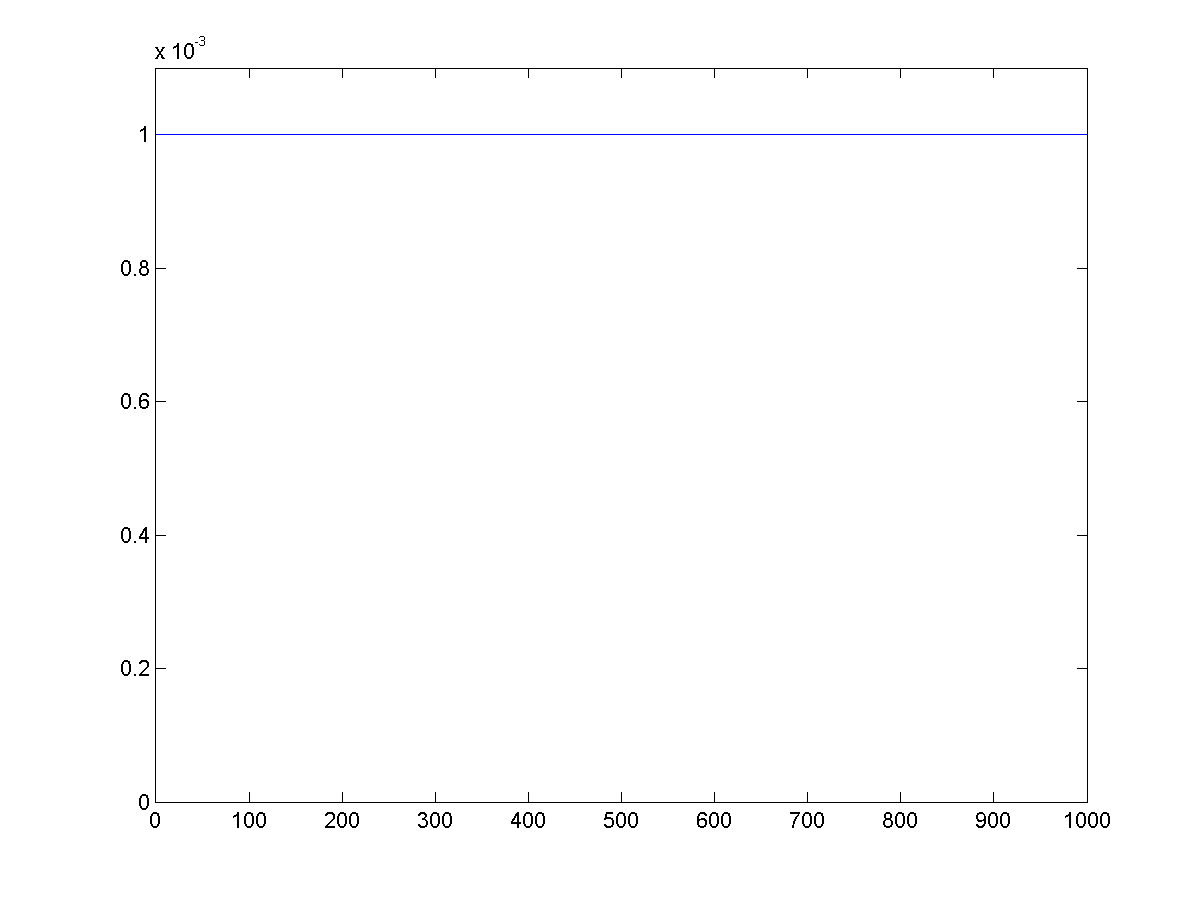
\includegraphics[width=\textwidth]{Paths/trc/plot-MLS-bel-1-8790226525.png}
                \caption{Beliefs in the starting state}
                \label{fig:bel_MLS_trc_part1}
                \hspace{10pt}
        \end{subfigure}
        \quad
        \begin{subfigure}{0.48\textwidth}
        		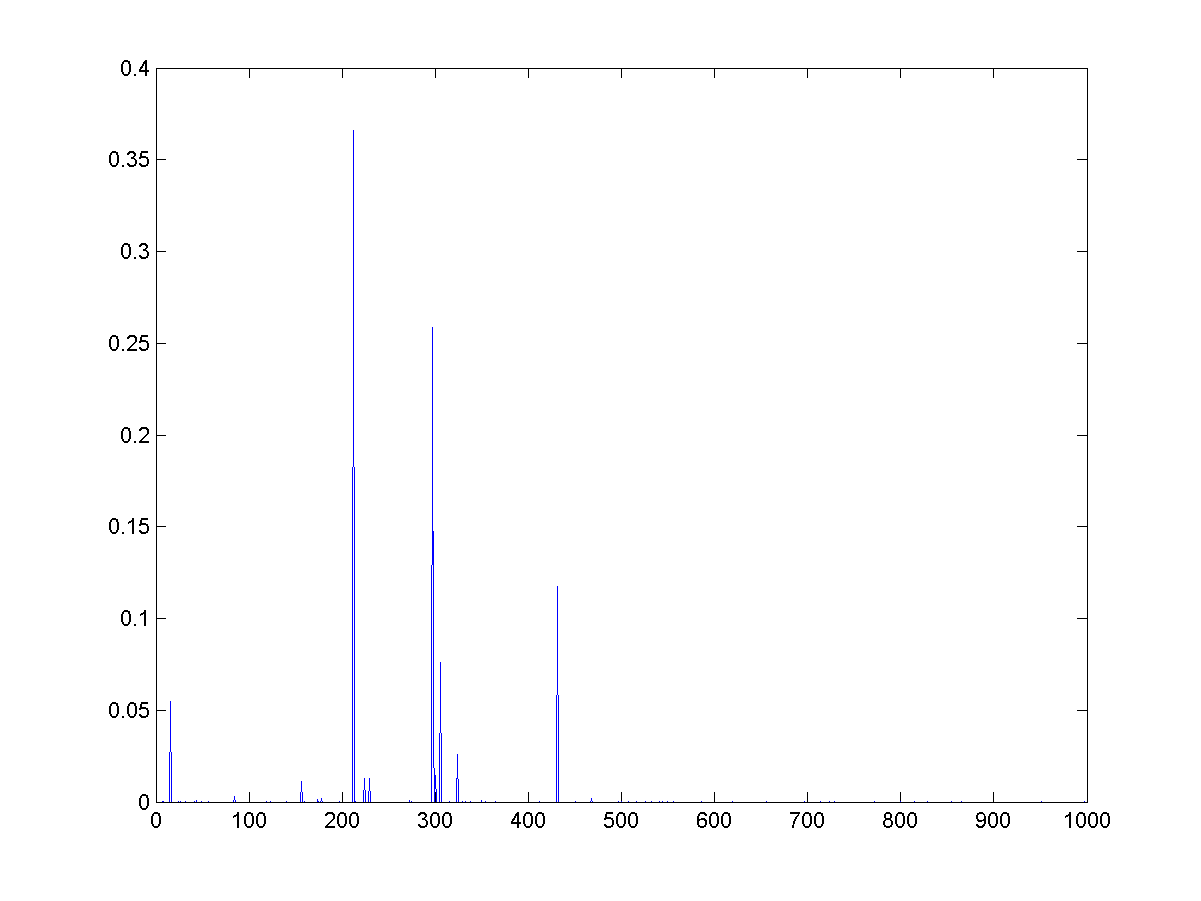
\includegraphics[width=\textwidth]{Paths/trc/plot-MLS-bel-2-8790226525.png}
                \caption{Beliefs in the 20th state}
                \label{fig:bel_MLS_trc_part2}
                \hspace{-10pt}
        \end{subfigure}
        \caption{The beliefs in the trc problem during an MLS run}
        \label{fig:bel_trc_MLS}
\end{figure}

\begin{figure}
        \centering
        \begin{subfigure}{0.48\textwidth}
        		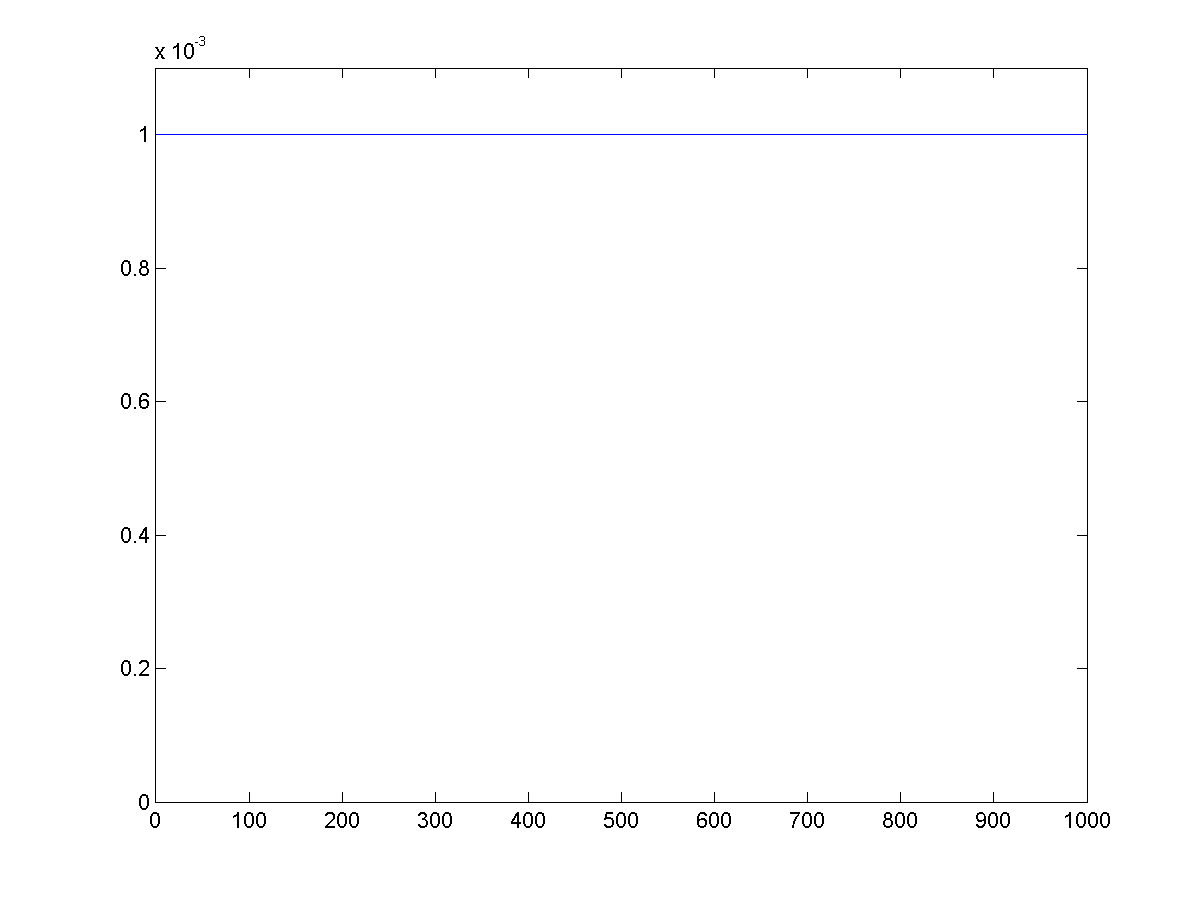
\includegraphics[width=\textwidth]{Paths/trc/plot-QMDP-bel-1-8790226525.png}
                \caption{Beliefs in the starting state}
                \label{fig:bel_qmdp_trc_part1}
                \hspace{10pt}
        \end{subfigure}
        \quad
        \begin{subfigure}{0.48\textwidth}
        		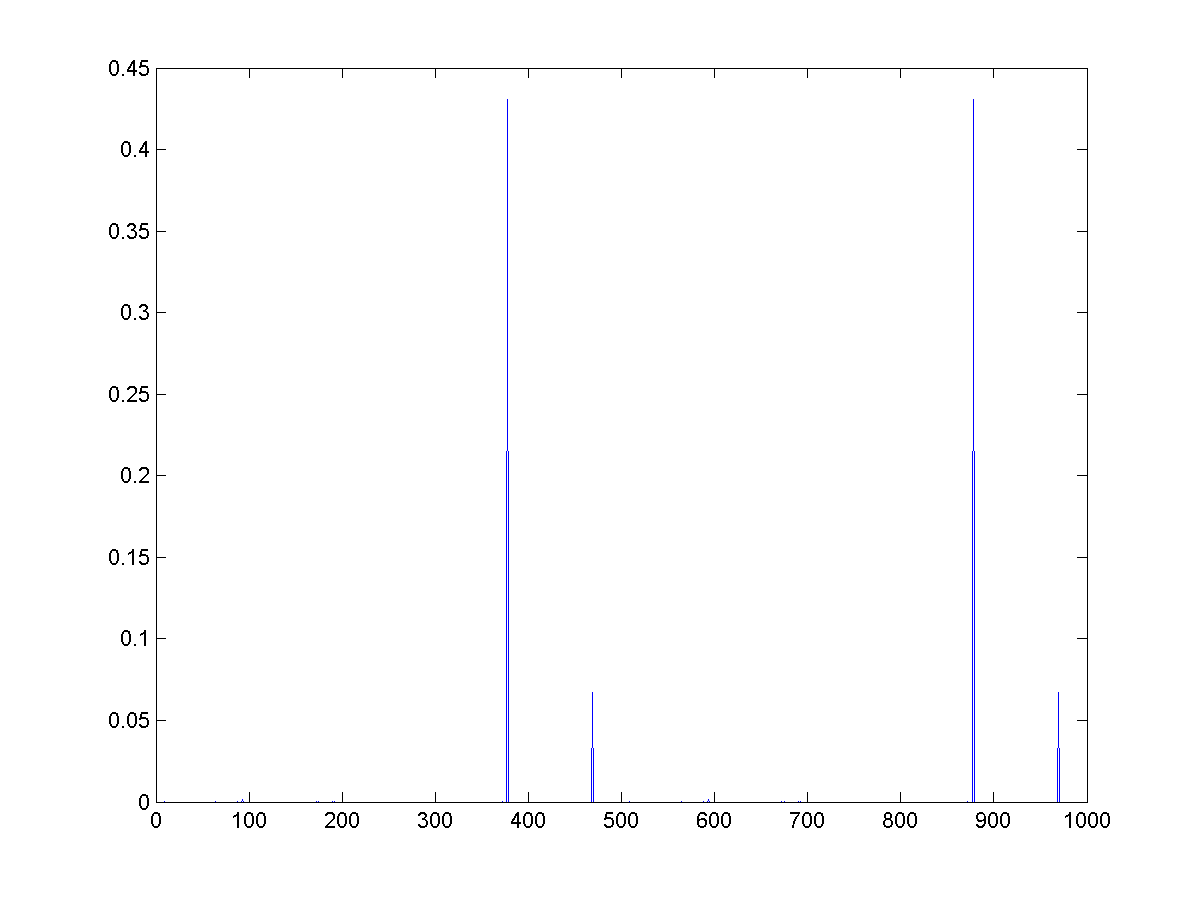
\includegraphics[width=\textwidth]{Paths/trc/plot-QMDP-bel-2-8790226525.png}
                \caption{Beliefs in the 20th state}
                \label{fig:bel_qmdp_trc_part2}
                \hspace{-10pt}
        \end{subfigure}
        \caption{The beliefs in the trc problem during a $Q_{MDP}$ run}
        \label{fig:bel_trc_QMDP}
\end{figure}

\begin{figure}
        \centering
        \begin{subfigure}{0.48\textwidth}
        		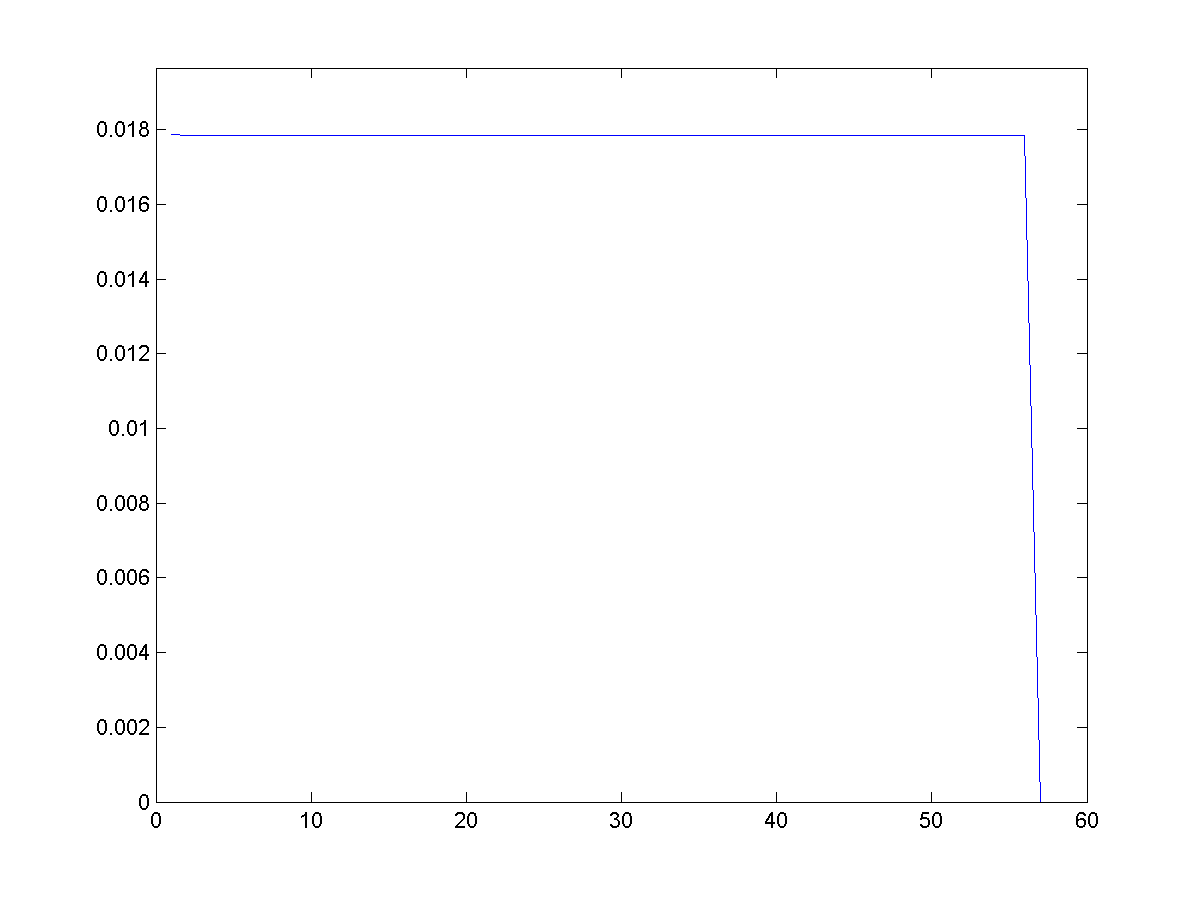
\includegraphics[width=\textwidth]{Paths/hallway/plot-QMDP-bel-1-8045708648.png}
                \caption{Beliefs in the starting state}
                \label{fig:bel_qmdp_hallway_part1}
                \hspace{10pt}
        \end{subfigure}
        \quad
        \begin{subfigure}{0.48\textwidth}
        		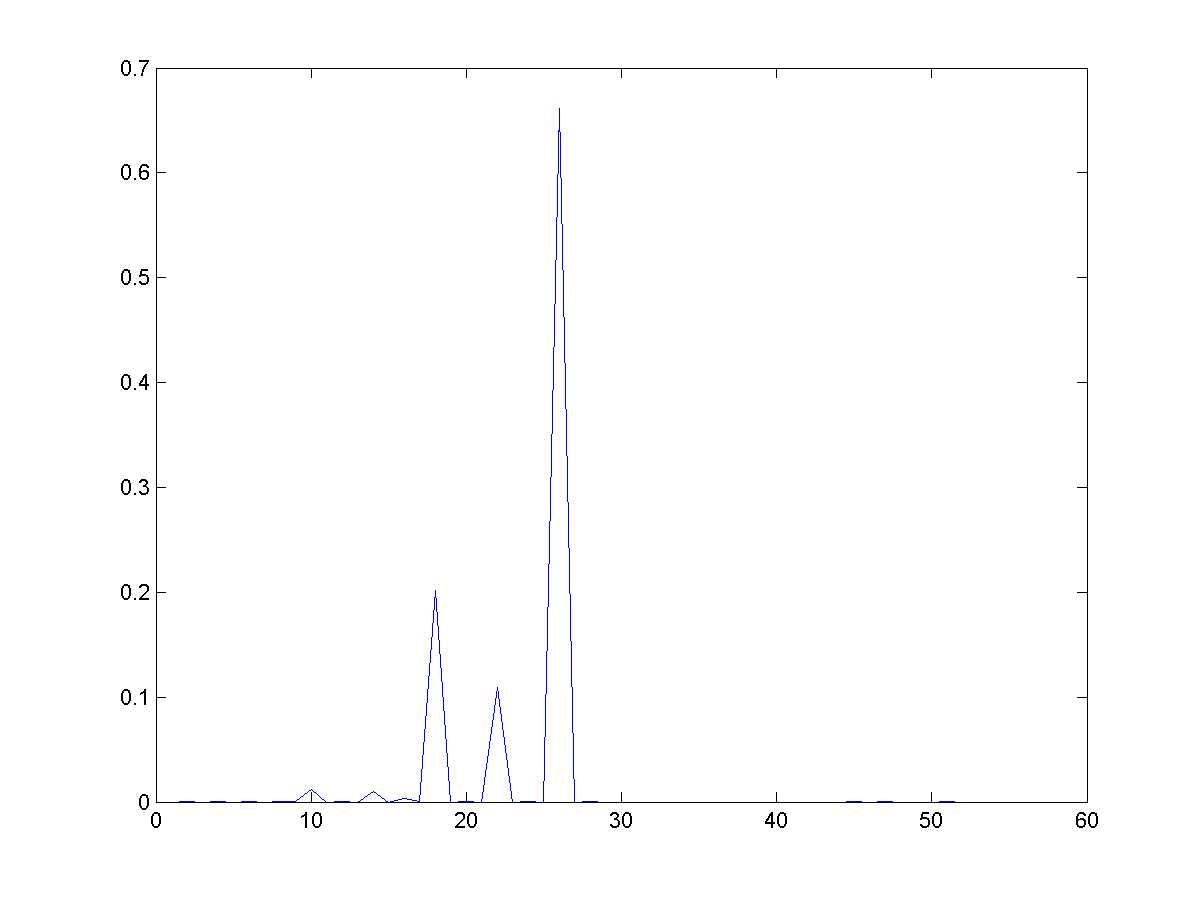
\includegraphics[width=\textwidth]{Paths/hallway/plot-QMDP-bel-2-8045708648.png}
                \caption{Beliefs in the 20th state}
                \label{fig:bel_qmdp_hallway_part2}
                \hspace{-10pt}
        \end{subfigure}
        \caption{The beliefs in the hallway problem during a successful $Q_{MDP}$ run}
        \label{fig:bel_hallway_QMDP}
\end{figure}

\restoregeometry

%%%%%%%%%%%%%%%%%%%%%%%%%%%%%%%%%%%%%%%%%%%%%
%											%
%				Heuristic					%
%											%
%%%%%%%%%%%%%%%%%%%%%%%%%%%%%%%%%%%%%%%%%%%%%

\section{Partially observable environments: heuristic methods}

In table \ref{table:rewards} a comparison between the different algorithms can be seen, with averages and standard deviation over 100 runs, each with a horizon of 100 steps.
While the fully observable case produces high reward values with a relatively small standard deviation, the MLS and $Q_{MDP}$ implementations output lower and much more varied results.

The $Q_{MDP}$ implementation often stalls during execution when a state is reached where staying in the current state is the best available action.
An extreme example here is the result achieved (or clear lack thereof) with the trc problem, where not a single run produced a reward. The evolution of the states in one such run is seen on figure \ref{fig:trc_qmdp} (a) and (b).

An explanation for the MLS and $Q_{MDP}$ behaviour as compared to the fully observable case is the fact that operation in a partially observable environment lacks total information and thus can't always calculate the best possible course of actions.\\
\\
A short visualization of the evolution of beliefs in both the MLS and $Q_{MDP}$ implementation for the trc problem can be seen in figures \ref{fig:bel_trc_MLS} and \ref{fig:bel_trc_QMDP}.
The $Q_{MDP}$ case clearly shows to equal sets of peaks, which causes the stalling mentioned earlier.
A similar visualization for the hallway problem using the $Q_{MDP}$ implementation and a run that did actually finish can be seen in figure \ref{fig:bel_hallway_QMDP}

%%%%%%%%%%%%%%%%%%%%%%%%%%%%%%%%%%%%%%%%%%%%%
%											%
%				Point-based					%
%											%
%%%%%%%%%%%%%%%%%%%%%%%%%%%%%%%%%%%%%%%%%%%%%

\section{Partially observable environments: point-based methods}

A performance comparison of the point-based Perseus algorithm and the $Q_{MDP}$ and MLS implementations was done using the hallway2 problem.
An overview can be seen in table \ref{table:performance}, where $Pers_{\bigotimes}$ represents the execution of the Perseus algorithm with different sampling parameters

This table demonstrates a clear difference between the relevant algorithms. \todo{Perseus10 sneller, Perseus100+ langer. Reward minder voor minder samples, maar veeeeeeel sneller. Zeggen of het nu beter of slechter is dan heuristical.}

\begin{table}
\centering
\begin{tabular}{ c || c | c | c | c | c | c | c}
\hfill & MLS & $Q_{MDP}$ & $Pers_{10}$ & $Pers_{100}$ & $Pers_{1000}$ & $Pers_{10000}$ \\
\hline
$\mu_{Reward}$ & 0.1896 & 0.09883 & 0.1548 & 0.2497 &  0.2473 & 0.23379\\
$\sigma_{Reward}$ & 0.1688 & 0.2166 & 0 & 0.007125 & 0.004098 & 0.006262 \\
\hline \hline
$\mu_{Runtime}$  & 2.746 & 2.675 & 2.1368 &  55.57 & 61.99 & 69.63 \\
$\sigma_{Runtime}$  & 0.01467 & 0.014556 & 0.2102 & 0.3610 & 0.9568 & 2.4624 \\
\end{tabular}
\caption{Performance of the different algorithms for the hallway2 problem}
\label{table:performance}
\end{table}

\todo{Based on 5 iterations for perseus}.

%%%%%%%%%%%%%%%%%%%%%%%%%%%%%%%%%%%%%%%%%%%%%
%											%
%					Part II					%
%											%
%%%%%%%%%%%%%%%%%%%%%%%%%%%%%%%%%%%%%%%%%%%%%

\part{}

%%%%%%%%%%%%%%%%%%%%%%%%%%%%%%%%%%%%%%%%%%%%%
%											%
%				Multi-agent					%
%											%
%%%%%%%%%%%%%%%%%%%%%%%%%%%%%%%%%%%%%%%%%%%%%

\section{Multi-agent planning under uncertainty}

\subsubsection*{Comparison between multi-agent problems solved with MMDP}
\todo{images invoegen!}
multi betekenent samen denken, single apart, 3x2 paden uitgetekend in todo folder. SINGLE -> NOG NIET HIER UITWERKEN

3 timings steeds omdat multi gedeelte met 2 vi's, single is apart.

\subsubsection*{Performance comparison between Single-agent and Multi-agent implementations}

\todo{figuurtjes met single-agent}

\todo{performance verschillen}

\todo{collision avoidance:
3) Query position+intention of other robot, clear priority between robots.
2) Look in 3x3 (for onedoor) + clear priority between robots.
1) Dynamic programming -> Alle states waarbij mogelijks zelfde toestand prunen. (hier niet al te veel states die gaan wegvallen, nie heel efficient.)}

%%%%%%%%%%%%%%%%%%%%%%%%%%%%%%%%%%%%%%%%%%%%%
%											%
%				Final Remarks				%
%											%
%%%%%%%%%%%%%%%%%%%%%%%%%%%%%%%%%%%%%%%%%%%%%

\part{}

%%%%%%%%%%%%%%%%%%%%%%%%%%%%%%%%%%%%%%%%%%%%%
%											%
%			Overview of Algorithms			%
%											%
%%%%%%%%%%%%%%%%%%%%%%%%%%%%%%%%%%%%%%%%%%%%%

\section{Overview of Algorithms}

\subsubsection*{Value Iteration}
There scripts can be found in the folder \texttt{yourcode\_new}.
\begin{itemize}
	\item \emph{vi.m}: The basic value iteration for single agent problems. It is optimized by using the build-in function \texttt{find} so it only iterates over the non-zero elements of the transition matrix.
	\item \emph{vi\_2.m}: A small optimization on vi.m by calculating the non-zero before and using these cached values for further calculations. 
	\item \emph{viMultiAgent.m}: The modification of vi\_2.m towards multiple agents because the non-existing of specific field in the problem structure.
	\item \emph{viMultiAgent2.m}: A significant modification on viMultiAgent so it transforms the transition matrix into a sparse matrix.
	\item \emph{viMultiAgentSingle.m}: The modification of vi\_2.m so the value iteration can calculate the different Q matrix for every single robot in a single script. 
	
\end{itemize}

\subsubsection*{Sample trajectory}
There scripts can be found in the folder \texttt{yourcode\_new}.
\begin{itemize}
	\item \emph{sampleTrajectories.m}: The basic trajectory sampler for single agents, working with full knowledge of the environment. The robot knows it exact location in every step.
	\item \emph{sampleTrajectoriesWithBeliefsMLS.m}: The trajectory sampler for single agents, working with a certain belief of his position in the environment. The choice of the action is based on the most likely state, which is named MLS.
	\item \emph{sampleTrajectoriesWithBeliefsQMDP.m}: The trajectory sampler for single agents, working with a certain belief of his position in the environment. The choice of the action is based on the beliefs, which is named $Q_{MDP}$.
	\item \emph{sampleTrajectoriesMultiAgents.m}: The trajectory sampler for multiple agents with a combined knowledge of the environment. Also no beliefs are introduced in this problem.
	\item \emph{sampleTrajectoriesMultiAgentsSingle.m}: The trajectory sampler for multiple agents with no combined knowledge of the environment. Also no beliefs are introduced in this problem.
\end{itemize}

The reward coming from following a certain path can be afterwards calculated based on the sequence of states and actions. An example can be found in the scripts \texttt{calculating\_rewards.m} and \texttt{calculating\_rewards.m} in the folder \texttt{yourcode\_graphical\_scripts}.

\subsubsection*{Graphical scripts}
All the scripts used for generating the images and data in this report can be found in the folder \texttt{yourcode\_graphical\_scripts}.

%%%%%%%%%%%%%%%%%%%%%%%%%%%%%%%%%%%%%%%%%%%%%
%											%
%				Time Spent					%
%											%
%%%%%%%%%%%%%%%%%%%%%%%%%%%%%%%%%%%%%%%%%%%%%

\section{Time Spent}
Most of the time spent on this project was done cooperatively and thus the effort is distributed quite evenly.
Based on combined agenda's we estimate both having spent between 28 and 35 hours on this project. 
This does not include the many hours it took to generate some images and statistics over several runs in the more expansive problems.


\end{document}
